%%%%%%%%%%%%%%%%%%%%%%% file template.tex %%%%%%%%%%%%%%%%%%%%%%%%%
%
% This is a general template file for the LaTeX package SVJour3
% for Springer journals.          Springer Heidelberg 2010/09/16
%
% Copy it to a new file with a new name and use it as the basis
% for your article. Delete % signs as needed.
%
% This template includes a few options for different layouts and
% content for various journals. Please consult a previous issue of
% your journal as needed.
%
%%%%%%%%%%%%%%%%%%%%%%%%%%%%%%%%%%%%%%%%%%%%%%%%%%%%%%%%%%%%%%%%%%%
%
% First comes an example EPS file -- just ignore it and
% proceed on the \documentclass line
% your LaTeX will extract the file if required
\begin{filecontents*}{example.eps}
%!PS-Adobe-3.0 EPSF-3.0
%%BoundingBox: 19 19 221 221
%%CreationDate: Mon Sep 29 1997
%%Creator: programmed by hand (JK)
%%EndComments
gsave
newpath
  20 20 moveto
  20 220 lineto
  220 220 lineto
  220 20 lineto
closepath
2 setlinewidth
gsave
  .4 setgray fill
grestore
stroke
grestore
\end{filecontents*}
%
\RequirePackage{fix-cm}
%
%\documentclass{svjour3}                     % onecolumn (standard format)
%\documentclass[smallcondensed]{svjour3}     % onecolumn (ditto)
\documentclass[smallextended]{svjour3}       % onecolumn (second format)
%\documentclass[twocolumn]{svjour3}          % twocolumn
%
\smartqed  % flush right qed marks, e.g. at end of proof
%
\usepackage{graphicx}
%
%
%
%\documentclass[envcountsame,envcountchap]{svmono}
%
\usepackage[latin1]{inputenc}
\usepackage[T1]{fontenc}
%\usepackage{graphicx}
\usepackage[bottom]{footmisc}
% places footnotes at page bottom
\usepackage{algorithmic}
\usepackage{algorithm}

\newcommand{\icm}{ICM}
\newcommand{\ibm}{IBM}
\newcommand{\prog}{\emph{3DHit}}



\begin{document}


\title{3D-Hit: fast structural comparison of proteins on multicore architectures}
\label{DPlewczynski} % Always give a unique label
%\thanks{Grants or other notes
%about the article that should go on the front page should be
%placed here. General acknowledgments should be placed at the end of the article.}
%}
%\subtitle{Do you have a subtitle?\\ If so, write it here}

%\titlerunning{Short form of title}        % if too long for running head

\author{\L{}. Bieniasz-Krzywiec, \and 
M. Cytowski, \and 
L. Rychlewski, \and
D. Plewczynski       
%        Second Author %etc.
}

%\authorrunning{Short form of author list} % if too long for running head


%$^a$ Interdisciplinary Centre for Mathematical and Computational Modelling, \\
%University of Warsaw (ICM), 
%Pawi\'nskiego 5a, 02-106 Warsaw, Poland \\
%$^b$ Faculty of Mathematics, Informatics and Mechanics, University of Warsaw,\\ Banacha 2, 02-097 Warsaw, Poland, \\
%$^c$ BioInfoBank Institute, Limanowskiego 24A16, 60-744 Pozna\'n, Poland \\


\institute{D. Plewczynski, \L{}. Bieniasz-Krzywiec, M. Cytowski \at
Interdisciplinary Centre for Mathematical and Computational Modelling, \\
University of Warsaw (ICM),  \\
Pawi\'nskiego 5a, 02-106 Warsaw, Poland \\
              \email{darman@icm.edu.pl}           %  \\
%             \emph{Present address:} of F. Author  %  if needed
           \and
           L. Rychlewski \at
BioInfoBank Institute, \\
Limanowskiego 24A16, \\ 
60-744 Pozna\'n, Poland \\
}

\date{Received: date / Accepted: date}
% The correct dates will be entered by the editor


\maketitle

%
%
%
%
%
%\chapter{3D-Hit: fast structural comparison of proteins on multicore architectures}
%\label{DPlewczynski} % Always give a unique label
%
%
%\begin{flushright}
%-- Arxiv paper -- \\
%\end{flushright}
%
%\hspace{20 mm}
%
%\begin{center}
%\L{}. Bieniasz-Krzywiec$^a$$^,$$^b$, M. Cytowski$^a$, L. Rychlewski$^c$, D. Plewczynski$^a$ \\
%\end{center}
%\hspace{20 mm}
%
%\begin{flushleft} 
%$^a$ Interdisciplinary Centre for Mathematical and Computational Modelling, \\
%University of Warsaw (ICM), 
%Pawi\'nskiego 5a, 02-106 Warsaw, Poland \\
%$^b$ Faculty of Mathematics, Informatics and Mechanics, University of Warsaw,\\ Banacha 2, 02-097 Warsaw, Poland, \\
%$^c$ BioInfoBank Institute, Limanowskiego 24A16, 60-744 Pozna\'n, Poland \\
%\end{flushleft}

% \title{3D-Hit: fast structural comparison of proteins on multicore architectures}

%\address[ICM]{Interdisciplinary Centre for Mathematical and Computational Modelling, University of Warsaw (ICM),\\ Pawi\'nskiego 5a, 02-106 Warsaw, Poland}
%\address[MIMUW]{Faculty of Mathematics, Informatics and Mechanics, University of Warsaw,\\ Banacha 2, 02-097 Warsaw, Poland},
%\address[BioInfo]{BioInfoBank Institute,\\ Limanowskiego 24A16, 60-744 Pozna\'n, Poland},

%\author{\L{}. Bieniasz-Krzywiec {^{\it a,b}}, \\
%M. Cytowski {^{\it a}}, \\
%L. Rychlewski {^{\it c}},   \\     
%D. Plewczynski {^{\it a}}
%}


%\author{\L{}. Bieniasz-Krzywiec$^a$$^,$$^b$, M. Cytowski$^a$, L. Rychlewski$^c$, D. Plewczynski$^a$}
%\title{3D-Hit: fast structural comparison of proteins on multicore architectures\\
%{\small $^a$ Interdisciplinary Centre for Mathematical and Computational Modelling, \\
%University of Warsaw (ICM), 
%Pawi\'nskiego 5a, 02-106 Warsaw, Poland \\
%$^b$ Faculty of Mathematics, Informatics and Mechanics, University of Warsaw,\\ Banacha 2, 02-097 Warsaw, Poland, \\
%$^c$ BioInfoBank Institute,\\ Limanowskiego 24A16, 60-744 Pozna\'n, Poland }}
%
%
%\subtitle{-- PPAM 2011 conference paper --}
%\maketitle
%
%
% \maketitle

%%%%%%%%%%%%%%%%%%%%%%%%%%%%%%%%%%%%%%%%%%%%%%%%%%%%%%%%%%%%%%%%%%%%%%%%%%%%%%%%%%%%%%%%%%%%%%%%%%%%%%%%%%%%
\begin{abstract}
%%%%%%%%%%%%%%%%%%%%%%%%%%%%%%%%%%%%%%%%%%%%%%%%%%%%%%%%%%%%%%%%%%%%%%%%%%%%%%%%%%%%%%%%%%%%%%%%%%%%%%%%%%%%

3D-Hit is a well established method for rapid detection of structural similarities between proteins, which 
is widely used in various bioinformatics web servers
(MetaServer, GRDB, 3D-Fun, Rosetta, etc.). 
The algorithm decomposes proteins into set of overlaping segments of 9-13 residues, then tries to
match them using root mean square distance metric. The best aligned pairs of segments are selected as seeds for futher analysis. 
Those initial hits are expanded by iterative process in order to construct the global structural alignment by 
concatenating pairs of matching segments.
The method has the same accuracy as the other state-of-the-art structural comparison algorithms (LGscore2, DALI), yet it provides
much faster procesing times, and can be used in a high-throughput setup as the structural module of bioinformatics pipelines. 
The method is optimized in terms of speed and accuracy to work on  novel computer architectures, such as PowerXCell8i and Sun Constellation System. Here, we provide the source code of the 3D-Hit program, describe selected architectures on which the software was ported, 
present programing models, point out significant porting steps
and sumarize performance comparisons.

\keywords{proteins \and IBM Cell \and structure comparison \and bioinformatics \and optimization}
% \PACS{PACS code1 \and PACS code2 \and more}
% \subclass{MSC code1 \and MSC code2 \and more}


\end{abstract}

%%%%%%%%%%%%%%%%%%%%%%%%%%%%%%%%%%%%%%%%%%%%%%%%%%%%%%%%%%%%%%%%%%%%%%%%%%%%%%%%%%%%%%%%%%%%%%%%%%%%%%%%%%%%
\section{Introduction}
%%%%%%%%%%%%%%%%%%%%%%%%%%%%%%%%%%%%%%%%%%%%%%%%%%%%%%%%%%%%%%%%%%%%%%%%%%%%%%%%%%%%%%%%%%%%%%%%%%%%%%%%%%%%
The PowerXCell8i is a pioneering microprocessor architecture
supposed to bridge the gap between conventional desktop computers and
specialized high-performance machines.
It has been designed to support very wide range of applications.
The Cell processor consists of nine processor elements operating on a
shared and coherent memory.
Functions of those processors are specialized into two types, i.e., a 
\emph{PowerPC Processing Element} (PPE), which usually acts
as a controller and is designed to run operating system and 
eight \emph{Synergistic Processing Elements} (SPEs), which
handle computational workload and are optimized for SIMD code execution.
PowerXCell8i processors are usually available as a dual processor nodes within
the IBM QS22 blades.
This gives a shared memory programming environment with 16
computational cores.
Moreover due to its specific architecture, Cell processor achieves very good
performance results with relatively low power consumption (in terms of
performance per Watt).
As a result, \emph{Nautilus} \cite{nau} --- cluster of IBM QS22 blades based on
Cell processors installed at \emph{Interdisciplinary Centre for Mathematical and
Computational Modelling} (ICM) has been ranked as No. 1 in two editions of
The Green500 List \cite{g500} of the world most energy-efficient supercomputers.\\
The Sun Constellation System, another high-performance computer available at ICM,
is a cluster based on a x86 architecture.
This powerful machine consists of blades packed into special-purpose
racks, which are tied together with highly-efficient InfiniBand connections.
Each blade is equipped with four AMD Quad-Core Opteron 835X processors (which
gives 16 computational cores per blade) and up to 32 Gb of memory.\\
In this paper we describe two fast implementations of an efficient scanning
method for detecting structural similarities between proteins.
The first of them is an application designed for the PowerXCell8i processors.
The second takes advantage of OpenMP and therefore can be executed on
virtually all architectures providing shared memory access, including the Sun
Constellation System.
Thus, we compared two shared memory systems with different
architectures but the same number of computational cores.
The algorithm used in our programs  was originally created by Dariusz Plewczy\'nski
et al. \cite{3dhit1,3dhit2,3dhit3,3dhit4}\\
The original code, destined to execute on x86 architecture, was ported using two
different frameworks: Cell SDK with its SPE library (for PowerXCell8i
architecture) and OpenMP (for parallel computers with shared memory).
The Cell-accelerated application achieved an overall speedup of 12 over
single threaded version executing on 1 SPE core.
This level of performance was obtained with the use of all 16 SPU cores
available within IBM QS22 blade.
However, the program parallelized with OpenMP library performed even better in terms of the
final walltime achieved during benchmarking tests.
In the course of our work we encountered very interesting aspects of parallel
programming and learned how to identity parts of code whose performance
could benefit from novel high-performance architectures.

%%%%%%%%%%%%%%%%%%%%%%%%%%%%%%%%%%%%%%%%%%%%%%%%%%%%%%%%%%%%%%%%%%%%%%%%%%%%%%%%%%%%%%%%%%%%%%%%%%%%%%%%%%%%
\section{Structural alignment}
%%%%%%%%%%%%%%%%%%%%%%%%%%%%%%%%%%%%%%%%%%%%%%%%%%%%%%%%%%%%%%%%%%%%%%%%%%%%%%%%%%%%%%%%%%%%%%%%%%%%%%%%%%%%
It has been discovered that the three dimensional structure of a protein is more
conserved during the process of evolution than its primary sequence \cite{chle}.
Therefore, the comparison of 3D structures of two proteins makes it possible to
establish distant evolutionary relationships, even between very diverged proteins.
As a result, the 3D structural alignment of proteins increases our understanding of
more distant evolutionary relationships \cite{buj2000,jms}.
The correspondence between structural and functional classification enables
scientists to determine functions of various newly discovered folds and whole
protein families. Structural similarity can suggest evolutionary links between protein
families, which can result in more detailed functional annotation
of a given protein at molecular level.
Moreover, the structural comparison can guide the experimental structure
determination process, by tracing shifts in low resolution
models.
The aforementioned reasons make the structural alignment the 
very important part of bioinformatics every-day work.\\
On the other hand, the size of Protein Data Bank \cite{pdb} 
is growing rapidly doubling every 18 months.
This huge amount of structural data needs very fast and accurate computer programs to deal
with the extraction of structural information and comparison of the new proteins with the previously 
annotated ones.
Those programs should enable not only
structure-to-structure search, but also alignment over all proteins from the
whole database on a real time basis.
So far, such computations done has been performed by several state-of-the-art methods,
including \prog{} code.
Because of the overwhelming and constantly growing 
amount of processing to be performed, scientists requested
the support of the \emph{Joint Cell Competence Centre} \cite{jccc}.
Due to an ongoing collaboration between \icm{} and \ibm{}, it was decided to
port the \prog{} code, \emph{inter alia}, to the PowerXCell8i Architecture and use Cell
based machines as a computational facility.\\
The purpose of this article is to present how the \prog{} program has been
ported and tuned on novel architectures and how processing performance of
accelerated versions compares to the x86 implementation.

%%%%%%%%%%%%%%%%%%%%%%%%%%%%%%%%%%%%%%%%%%%%%%%%%%%%%%%%%%%%%%%%%%%%%%%%%%%%%%%%%%%%%%%%%%%%%%%%%%%%%%%%%%%%
\section{Overview of the algorithm}
%%%%%%%%%%%%%%%%%%%%%%%%%%%%%%%%%%%%%%%%%%%%%%%%%%%%%%%%%%%%%%%%%%%%%%%%%%%%%%%%%%%%%%%%%%%%%%%%%%%%%%%%%%%%
\prog{} program provides the structural alignment of two proteins.
It uses in-house customised version of the Smith-Waterman dynamic programing
algorithm combined with intensive three-dimensional rotation and translation
routines that align two geometrical objects in order to minimize the root mean square
distance computed for all heavy atoms from both proteins.
The flow chart of entire sequential program is presented in Figure \ref{fig:figureone}.
The most time consuming part of the code is the preparation of structural
alignment matrix which is carried out by the main loop of the program and is computed by examining local similarities between protein sequences. Alignment matrix is used at the end of the program, it serves as input data for the Smith-Waterman algorithm to compute the final global alignment of the whole proteins. 
To identify similarity substructures of two proteins, the program compares
parts of their chains with a fixed length of 256 amino acids
that we called \emph{segments}.
The \prog{} program analyses structural similarities between each pair of segments through two successive steps (see pseudo-code of Algorithm 1).\\
First, it decides whether central parts of segments, which we call
\emph{seeds}, are similar enough to proceed with further computations.
Seeds are very short subsequences with 13 amino acids.
The \prog{} algorithm makes rotations and translations of alpha carbon atoms of both seeds in
order to minimize the root mean square deviation (RMSD) between them.
Second, if the structural similarity of the two seeds is high enough,
the algorithm starts to analyze two longer continuous parts of the main chains
centered on seeds.
It uses a rotation matrix and a translation vector for a Cartesian-space
superimposition of the two seeds to rotate and translate these large segments.
Next, it defines the similarity matrix for the dynamic programming in the
following way.
If two alpha carbon atoms taken from the superimposed large segments are close enough
in space (below 3A), it assigns 1 to their similarity score or 0, otherwise.
Then alignment score based on such similarity score matrix is computed.
If the alignment score is large enough, algorithm passes this pair of segments
on to the next filter.
The whole procedure is repeated for subsequences of 100, 200 and 256
amino acids centered on seeds.\\
For each pair of segments, the resulting score -- number of superimposed alpha carbon atoms in the aligned segments -- is recorded in an
additional final alignment matrix.
At the end, this final matrix is used to find the best alignment of whole proteins.
If no pair of segments did pass the filter sequence just described, the overall score is set to 0.
\begin{figure}[h]
\centering{
%\resizebox{0.5\textwidth}{!}{
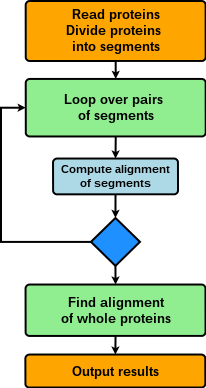
\includegraphics[scale=0.35]{3dhitScalar.png}
}
%}
\caption{The flow chart of the scalar (starting) version of the 3D-Hit program.} \label{fig:figureone}
\end{figure}

%\begin{algorithm}
%\caption{A~sketch of the structural alignment algorithm}
%
%\begin{tabular}{lp{13.39cm}}
%{\em Input:} &
%Two protein sequences: \texttt{protein1} and \texttt{protein2}.\\
%{\em Output:} &
%Structural alignment of the given proteins.\\
%\end{tabular}
%
%\begin{enumerate}
%\item
%Divide each protein into segments of fixed length (256 amino acids).
%
%\item 
%\begin{verbatim}
%// Create a structural alignment matrix containing similarity
%// scores between each pair of segments.
%\end{verbatim}
%For each \texttt{segment1} in \texttt{protein1} and \texttt{segment2} in \texttt{protein2},
%compute the number of superimposed Calpha atoms in the aligned pair of segments:
%\begin{verbatim}
%    similarityMatrix[segment1, segment2] =
%        ComputeAlignmentOfSegments(segment1, segment2)
%\end{verbatim}
%
%\item
%Find alignment of the whole proteins by running Smith-Waterman algorithm on them with the \texttt{similarityMatrix} as an input.
%
%\end{enumerate}
%\end{algorithm}

\begin{algorithm}
\caption{\texttt{ComputeAlignmentOfSegments(segment1, segment2)}}

\begin{tabular}{lp{13.39cm}}
{\em Input:} &
Two segments of potein sequences.\\
{\em Output:} &
The number of superimposed Calpha atoms in the aligned segments.\\
\end{tabular}

\begin{enumerate}
\item
Extract the seed of each segment (seed is the central part of segment consisting of 13 amino acids).
Find the rotation matrix and the translation vector minimizing the RMSD between the two seeds.
If the optimal RMSD is too low, exit and return 0.

\item
For \texttt{len} in \{100, 200, 256\}:
\begin{itemize}
\item[(4a)]
Define the subsequences to consider:\\
\begin{tabular}{lp{8cm}}
\texttt{subsequence1 =} &
the subsequence of length \texttt{len} surrounding the seed of \texttt{segment1}. \\
\texttt{subsequence2 =} &
the subsequence of length \texttt{len} surrounding the seed of \texttt{segment2}. \\
\end{tabular}

\item[(4b)]
Align the two subsequences using the rotation matrix and the translation vector computed in the previous step.

\item[(4c)]
\begin{verbatim}
// Define the alignment matrix for the two subsequences:
\end{verbatim}
For each \texttt{atom1} in \texttt{subsequence1} and \texttt{atom2} in \texttt{subsequence2}:
\begin{verbatim}
    alignmentMatrix[atom1, atom2] = 
        distance(atom1, atom2) < 3A ? 1 : 0
\end{verbatim}

\item[(4d)]
Find the alignment of subsequences by running Smith-Waterman algorithm on them with the \texttt{alignmentMatrix} as an input.

\item[(4e)]
If computed alignment is better than the one found previously, continue the loop. Otherwise, return the best alignment found previously.

\end{itemize} 

\end{enumerate}
\end{algorithm}



%%%%%%%%%%%%%%%%%%%%%%%%%%%%%%%%%%%%%%%%%%%%%%%%%%%%%%%%%%%%%%%%%%%%%%%%%%%%%%%%%%%%%%%%%%%%%%%%%%%%%%%%%%%%
\section{Porting process}
%%%%%%%%%%%%%%%%%%%%%%%%%%%%%%%%%%%%%%%%%%%%%%%%%%%%%%%%%%%%%%%%%%%%%%%%%%%%%%%%%%%%%%%%%%%%%%%%%%%%%%%%%%%%
After profiling the original version of the \prog{} program we found out that
the most time consuming part of the code was a function implementing algorithm,
which compares two given segments.
Intrinsically, the algorithm was executed in sequence with each pair of segments as a
parameter.
As a result, program spent more than $90\%$ of its time in that function.
We decided to accelerate that program section by a parallelization process based on the libspe2 library model for Cell and the OpenMP model for x86 architectures.

\subsection{Parallel scheme}
Computations for each pair of segments can be performed independently with
no communication occurring between working threads.
Nevertheless, at the end the main thread must collect all partial results for
each pair of segments and compute the final result based on them.
We wondered whether those extra computation steps performed on partial results
would cause a new bottleneck.
In the case of the Cell implementation, the final result computing is handled by the PPE.
In the case of OpenMP version, the final result is processed by the master thread.
Fortunately, it turned out that accelerated versions of \prog{}
program spends only a fraction of percent of their execution times computing
final result.

\subsection{PowerXCell8i implementation}
We used the Cell SDK and its SPE library to implement this simple parallel
scheme.
The PPE processor executes the main application thread.
Its role is to read and preprocess the two protein sequence descriptions, create
SPE contexts, run appropriate working threads, collect partial results and
finally compute and return the final score and alignment.
Each SPE processor gets its set of segment pairs.
Then, it consecutively loads the descriptions of two segments into local memory space (Local Store) for each pair of segments from the set, executes function comparisons and stores the result back into main memory.

\subsubsection{Memory issue}
Porting most of the scientific applications to SPE processor is a rather challenging task
because of the size limitation of Local Store, which is only 256 KB.
This small space must be wisely administrated, because it has to accommodate
both program instructions and operating data.
Moreover, the only way to load and store data to and from Local Store is a Direct Memory Access (DMA)
mechanism.
It gives programmer a great deal of control, but on the other hand it is not
simple to use.\\
The \prog{} code is unfortunately memory consuming.
In the original version each execution of comparing algorithm requires memory
for at least $256^2$ floating point numbers and $256^2$ short integer values.
It is of course too much for the Local Store.
That is why we had to perform some memory optimizations including compression
and introduction of bit operations.
The resulting code was slightly slower and less accurate than the original one, however
thanks to those sacrifices, we were able to fit our program to Local Store.

\subsubsection{SIMD optimizations}
In its original version, \prog{} program spends nearly
$30\%$ of its execution time calculating rotation matrices and translation
vectors for Cartesian-space superimposition of pairs of segments.
The part of code responsible for that task turned out to be a good candidate for
a vectorization process due to the quantity of simple algebraic operations.\\
First of all, we decided to take advantage of the auto SIMDizing abilities of \texttt{GCC} compiler by switching on option \texttt{-ftree-vectorize}.
At first, it did not help much since the code was too complex
to allow the automatic analysis by the compiler.
Therefore, we followed the guidelines proposed in \cite{rb} to simplify the code.\\
Even after using specific compiler directives, the compiler was still unable to automate loop vectorization.
We decided to tune the remaining parts of code manually by instruction
substitution.
The main vector operations used in the SPE computational kernel were
\texttt{spu\_add}, \texttt{spu\_mul}, \texttt{spu\_madd} and
\texttt{spu\_splats}.
All of these instructions were operating on float 4 entry vectors, so we could
speed up the vectorized loops of the appropriate steps of the algorithm by a factor of about
4 times.
The result of this effort is presented in Tab.~\ref{tab:t1}.

\begin{table}[htb]
\begin{footnotesize}
\caption{Performance results of SIMD and noSIMD versions.}
\label{tab:t1}
\newcommand{\m}{\hphantom{$-$}}
\newcommand{\cc}[1]{\multicolumn{1}{c}{#1}}
\renewcommand{\tabcolsep}{0.5pc} % enlarge column spacing
\renewcommand{\arraystretch}{1.2} % enlarge line spacing
\begin{tabular}{@{}llll}
\hline
\textbf{Version} & \textbf{Compiler} & \textbf{Average time} & \textbf{Speedup} \\
\hline
% AMD Opteron, noSIMD, 1 core & \texttt{GCC} (no optimizations) & 1.435 s & X \\
PowerXCell8i, noSIMD, 1 SPE & \texttt{GCC} (\texttt{-O3}) & 1.546 & 1.0 \\
PowerXCell8i, noSIMD, 16 SPEs & \texttt{GCC} (\texttt{-O3}) & 0.181 s &  8.541 \\
PowerXCell8i, SIMD, 16 SPEs & \texttt{GCC} (\texttt{-O3 -ftree-vectorize}) & 0.164 s & 9.427 \\
\hline
\end{tabular}\\[2pt]
\end{footnotesize}
\end{table}

\subsubsection{Efficient implementation of the parallel scheme}
In our first approach to implement chosen parallel scheme, we met very
interesting problem.
At the beginning we were assigning jobs for the computational kernels
arbitrarily.
Each SPE program was given a consecutive sequence of pairs of segments to
operate on.
Nevertheless, it was a wrong decision because of the inefficient load balancing.
As described before, the algorithm for comparing segments does not always behave in the same manner.
For example, the algorithm may finish very quickly if seeds have poor similarity rate.
Moreover, cutoffs may occur at the every stage, including analysis of longer
segments.
That is why it is important to assign each SPE with more or less the same
amount of real work, which may not necessarily mean the same amount of pairs of
segments.\\
We tried many different ways to fulfil this requirement.
First of all, we decided to divide the whole set of tasks into 16 random subsets
on the PPE side of application.
Each SPE program operated on one of those randomly chosen work packages.
This solution allowed the achievement of a very good load balancing,
but let, on the other hand, to a drastic slowing down in the rate of PPE thread processing resulting in an unsustainable increase of time execution of about $15\%$.\\
By contrast, the use of PPE thread as a management
resource allow the workload to be distributed coherently according to computations needs.
In this approach each idle SPE asks PPE for a new package for processing.
We implemented and tested a few versions of such processing model by taking advantage of SPE mailboxes
as well as advanced DMA transfers with double buffering.
Unfortunately non of them met our expectations, because of the slowdown caused
by the increase in communication load.\\
In the last approach, we have decided to choose an arbitrary random  permutation and assign it statically to each SPE kernel as a constant.
It allowed us the complete eradication of communication bottlenecks between PPE and SPE and
to achieve reasonable load balancing.
The performance comparison of all of these methods is presented in
Tab.~\ref{tab:t2}.

\begin{table}[htb]
\begin{footnotesize}
\caption{Performance results of various versions of work load management for the SPE threads.}
\label{tab:t2}
\newcommand{\m}{\hphantom{$-$}}
\newcommand{\cc}[1]{\multicolumn{1}{c}{#1}}
\renewcommand{\tabcolsep}{0.5pc} % enlarge column spacing
\renewcommand{\arraystretch}{1.2} % enlarge line spacing
\begin{tabular}{@{}lll}
\hline
\textbf{Version} & \textbf{Compiler} & \textbf{Average time} \\
\hline
% Original, AMD Opteron, 1 core & \texttt{GCC} (no optimizations) & 1.435 s \\
Randomization on PPE, 16 SPEs & \texttt{GCC} (\texttt{-O3 -ftree-vectorize}) & 0.247 s \\
Dynamic distribution, 16 SPEs & \texttt{GCC} (\texttt{-O3 -ftree-vectorize}) &  0.370 s \\
Static permutation, 16 SPEs & \texttt{GCC} (\texttt{-O3 -ftree-vectorize}) & 0.164 s \\
\hline
\end{tabular}\\[2pt]
\end{footnotesize}
\end{table}

\subsubsection{Other optimizations}
Each SPE program is executed once at the beginning and serves as a computational
facility for many tasks.
Thanks to that we are able to eliminate time needed for SPE context creation.
In addition, we used the DMA double buffering
mechanism.
While SPE is carrying on computations, its Memory Controller can coherently load
the next portions of data from the main memory.
This simple idea allowed us to overlap main memory load and store operations with computations.\\
In comparison to the single SPE, we achieved an overall speedup of 6.14 while
executing on 8 SPEs and 9.39 while executing on 16 SPEs.
In addition, running two parallel instances of the \prog{} program, each using 8 SPEs, on the QS22 server equipped with two Cell chips allowed us to reach an average speedup of 12.

\begin{figure}[h]
\centering{
\resizebox{0.9\textwidth}{!}{
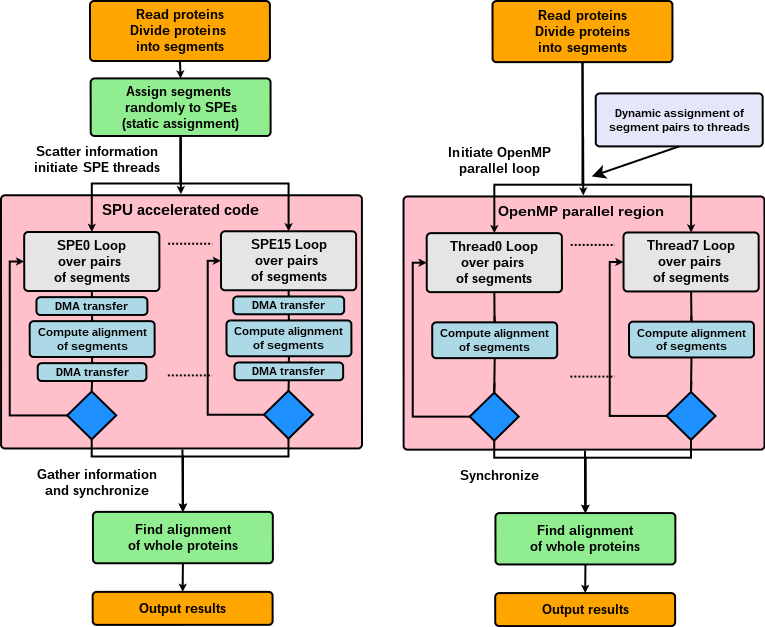
\includegraphics{3dhitParallel.png}
}
}
\caption{The flow charts of the PowerXCell8i (left) and OpenMP (right) parallel versions of the 3D-Hit program. Important features of both implementations are indicated in the picture.} \label{fig:figuretwo}
\end{figure}

\subsection{OpenMP implementation}
The implementation of a programming model based on OpenMP is very simple.
The whole set of pairs of segments is dynamically (and automatically)
distributed among OpenMP threads.
Each such a thread executes an algorithm similar to the one described in the 
PowerXCell8i's section.
It gets a pair of segments, computes an answer and stores the result in the
specified place in the main memory.\\
In spite of its simplicity, the OpenMP implementation of our application
appeared to be very efficient and accurate.
In comparison to the single-threaded version, we achieved an overall speedup of
4.37 while executing on 8 cores.
Taking advantage of the same schema as the one used with PowerXCell8i
processors, we ran two parallel instances of \prog{} program, each using 8
threads, on blades equipped with 16 processor units, which
gave an average speedup of 8.5 over the initial x86 version.

%%%%%%%%%%%%%%%%%%%%%%%%%%%%%%%%%%%%%%%%%%%%%%%%%%%%%%%%%%%%%%%%%%%%%%%%%%%%%%%%%%%%%%%%%%%%%%%%%%%%%%%%%%%%
\section{Performance results}
%%%%%%%%%%%%%%%%%%%%%%%%%%%%%%%%%%%%%%%%%%%%%%%%%%%%%%%%%%%%%%%%%%%%%%%%%%%%%%%%%%%%%%%%%%%%%%%%%%%%%%%%%%%%
\subsection{PowerXCell8i code analysis}
We have used a \texttt{spu\_timing} facility to analyze and tune the computational
kernels of the \prog{} Cell implementation.
Results presented in Tab.~\ref{tab:t3} and Tab.~\ref{tab:t4} show that we achieved
very good scaling over increasing number of working SPE threads.
The part of code that can be parallelized represents about $97.994\%$ of the execution
time spent by the single-threaded version of \prog{}.
We achieve an overall speedup of almost 9 that is only a little below the theoretical maximum expected by the Amdahl's Law, i.e. $\frac{1}{(1-0.97994) + \frac{0.97994}{16}}\approx12$.
The difference between observed and expected values is the most probably due to the use of built-in permutation of packages instead of actually randomly permutated set of segments. 
This approach increases the probability of occurrence of inefficient load balancing.
\begin{table}[htb]
\begin{footnotesize}
\caption{Profile results -- percentage of time spent in particular sections of the program.}
\label{tab:t3}
\newcommand{\m}{\hphantom{$-$}}
\newcommand{\cc}[1]{\multicolumn{1}{c}{#1}}
\renewcommand{\tabcolsep}{0.5pc} % enlarge column spacing
\renewcommand{\arraystretch}{1.2} % enlarge line spacing
\begin{tabular}{@{}llll}
\hline
\textbf{Part of code} & \textbf{1 SPE} & \textbf{8 SPEs} & \textbf{16 SPEs} \\
\hline
Preparing data & 0.004782 \% & 0.142613 \% & 0.359532 \% \\
Creating  SPE threads & 0.121318 \% & 7.627334 \% & 21.029137 \% \\
Waiting for threads & 97.844704 \% & 80.333420 \% & 62.397312 \% \\
Computing global result & 0.019680 \% & 0.139842 \% & 0.219315 \% \\
\hline
\end{tabular}\\[2pt]
\end{footnotesize}
\end{table}

\begin{table}[htb]
\begin{footnotesize}
\caption{Profile results -- absolute time spent in particular sections of the program.}
\label{tab:t4}
\newcommand{\m}{\hphantom{$-$}}
\newcommand{\cc}[1]{\multicolumn{1}{c}{#1}}
\renewcommand{\tabcolsep}{0.5pc} % enlarge column spacing
\renewcommand{\arraystretch}{1.2} % enlarge line spacing
\begin{tabular}{@{}llll}
\hline
\textbf{Part of code} & \textbf{1 SPE} & \textbf{8 SPEs} & \textbf{16 SPEs} \\
\hline
Preparing data & 0.000051 s & 0.000247 s & 0.000466 s \\
Creating  SPE threads & 0.001170 s & 0.012919 s & 0.027042 s \\
Waiting for threads & 1.492583 s & 0.207126 s & 0.114413 s \\
Computing global result & 0.000527 s & 0.000571 s & 0.000619 s \\
\hline
\end{tabular}\\[2pt]
\end{footnotesize}
\end{table}

\subsection{Performance Comparison}

We have designed a test to examine operational performance of \prog{} code
executing on various architectures.
We have chosen a set of 18 proteins from a database and compared execution times
on a Quad-Core AMD Opteron Processor 8354 based nodes and on a QS22 server.
Each pair of proteins from the test set was compared during a test run, which
gave us 324 single test cases.
The average results are presented in Tab.~\ref{tab:t5}.
\begin{table}[htb]
\begin{footnotesize}
\caption{Performance results on two systems: AMD Opteron 8354 and PowerXCell8i QS22.}
\label{tab:t5}
\newcommand{\m}{\hphantom{$-$}}
\newcommand{\cc}[1]{\multicolumn{1}{c}{#1}}
\renewcommand{\tabcolsep}{0.5pc} % enlarge column spacing
\renewcommand{\arraystretch}{1.2} % enlarge line spacing
\begin{tabular}{@{}llll}
\hline
\textbf{Architecture} & \textbf{Compiler} & \textbf{Time} & \textbf{Speedup} \\
\hline
AMD, 1 OpenMP thread & \texttt{GCC} (\texttt{-O3}) & 116.85 s & 1.00 \\
AMD, 4 OpenMP threads & \texttt{GCC} (\texttt{-O3}) & 38.22 s & 3.05 \\
AMD, 8 OpenMP threads & \texttt{GCC} (\texttt{-O3}) & 26.72 s & 4.37 \\
AMD, 16 OpenMP threads & \texttt{GCC} (\texttt{-O3}) & 26.09 s & 4.47 \\
\hline
PowerXCell8i, 1 SPE & \texttt{GCC} (\texttt{-O3 -ftree-vectorize}) & 499.07 s & 1.00 \\
PowerXCell8i, 8 SPEs & \texttt{GCC} (\texttt{-O3 -ftree-vectorize}) &  81.20 s & 6.14 \\
PowerXCell8i, 16 SPEs & \texttt{GCC} (\texttt{-O3 -ftree-vectorize}) & 53.14 s & 9.39 \\
\hline
\end{tabular}\\[2pt]
\end{footnotesize}
\end{table}
As we can see, the Cell accelerated version of \prog{} was approximately
two times slower than the OpenMP code executed on blades equipped with AMD
processors.
Those performance differences could be caused by disparities in technical
parameters of chosen machines.
According to our experiments, multiplication of two floating point scalars is
almost two times slower on PowerXCell8i SPE processors than on AMD Opterons.
Unfortunately a great deal of \prog{} code could not be vectorized and, as a
result, arithmetic operations on scalars are intense in our code.
Moreover, the PowerXCell8i version is slightly more complex.
For example, the necessity of performing a memory optimisations as described above is a bottleneck on its own.
Another very important feature that reduces the performance of the implemented SPU
kernels is a big number of branching introduced by the algorithm and a lack of
branch prediction mechanism within the SPU architecture.
As a result one of the most important computational parts of the code,
Smith-Waterman algorithm, is significantly slowed down on the Cell architecture.\\
On the other hand, the PowerXCell8i implementation has one desired feature, which
is unfortunately not a feature of OpenMP-based program, namely --- very good
scalability.
The reason of the bad scalability of OpenMP is probably due to the limited memory bandwidth when 16 working threads try to simultaneously read data from the shared memory
located on their blade, which results in a significant slowdown of data
transfer.
It should be stated here that the comparison of two longest sequences in the
benchmark test takes approximately only 0.22 seconds.
The memory bandwidth  is not a problem in PowerXCell8i implementation, due to
the presence of highly efficient Element Interconnect Bus (EIB), which provides
each SPE and its memory controller with private and very fast connection to the
main memory.

%%%%%%%%%%%%%%%%%%%%%%%%%%%%%%%%%%%%%%%%%%%%%%%%%%%%%%%%%%%%%%%%%%%%%%%%%%%%%%%%%%%%%%%%%%%%%%%%%%%%%%%%%%%%
\section{Summary}
%%%%%%%%%%%%%%%%%%%%%%%%%%%%%%%%%%%%%%%%%%%%%%%%%%%%%%%%%%%%%%%%%%%%%%%%%%%%%%%%%%%%%%%%%%%%%%%%%%%%%%%%%%%%
The current evaluation of \prog{} performed on dataset of circa 300 query proteins
reveals the quality of the tool, as compared with other programs. When compared
with DALI server, our tool is able to generate similar number of correct models, however
the final alignment quality is better in the case of the second service. In the 
case of distant structural comparisons, our method produced better ratings in all categories
(such as specificity analysis) when MaxSub evaluation method is used.
Concluding, the \prog{} software is on average less sensitive than the DALI
server, yet it is better than CE or VAST tools.\\
On the side of core optimizalization, we have ported the \prog{} 
program to the novel high-performance
architectures and achieved very good rate of speedup.
Our accelerated programs are planed to be embedded into the web application,
which will allow very fast and accurate mechanism for structural alignment of
proteins.
By taking advantage of PowerXCell8i and Quad-Core x86 novel architectures,
we were able to significantly reduce time of single computation and as a result
provide scientists all over the world with always up-to-date and fast tool for
structural alignment experiments.
The present version of our algorithm is very fast. It takes circa 2 seconds 
for a query protein of 500 amino acids to scan a database of 1000 templates.
The single comparison of two proteins with circa 500 amino acids 
is performed within a runtime of 0.002 seconds for \prog{}, where 
older version of the software took around 0.017 seconds. Other structural
alignment programs are significantly slower, CE takes 3 seconds to compare two
typical proteins, LGScore2 is around 6 seconds. \\
Because of its speed and portability (the source code is available from authors 
upon request) we believe that \prog{} program will continue to be widely used
in structural genomics projects, improving the structural comparison of  newly crystallized
proteins with large structural databases. We are planning to provide the internet web
server interface to the PDB database, in order to give user access to rapid structural 
alignment of its protein of interest with three-dimensional crystals or 3D models
of proteins. 
%%%%%%%%%%%%%%%%%%%%%%%%%%%%%%%%%%%%%%%%%%%%%%%%%%%%%%%%%%%%%%%%%%%%%%%%%%%%%%%%%%%%%%%%%%%%%%%%%%%%%%%%%%%%

\section{Acknowledgments}
%%%%%%%%%%%%%%%%%%%%%%%%%%%%%%%%%%%%%%%%%%%%%%%%%%%%%%%%%%%%%%%%%%%%%%%%%%%%%%%%%%%%%%%%%%%%%%%%%%%%%%%%%%%%
This work was supported by EC OxyGreen (KBBE-2007-212281) 6FP project as
well as the Polish Ministry of Education and Science (N301 159735,
and others).

\begin{thebibliography}{99}

\bibitem[1]{nau} Nautilus system,
http://cell.icm.edu.pl/index.php/Nautilus

\bibitem[2]{g500} The Green500 List,
http://www.green500.org/lists/2009/06/list.php

\bibitem[3]{3dhit1} Plewczynski D, Pas J, von Grotthuss M, Rychlewski L.
\textit{3D-Hit: fast structural comparison of proteins.}
Appl Bioinformatics. 2002;1(4):223-5.

\bibitem[4]{3dhit2}  Plewczynski D, Pas J, Von Grotthuss M, Rychlewski L.
\textit{Comparison of proteins based on segments structural similarity.}
Acta Biochim Pol. 2004;51(1):161-72.

\bibitem[11]{3dhit3} Plewczynski D, Rychlewski L, Jaroszewski L, Ye Y, Godzik A.
\textit{SEA and FRAGlib - an Integrated Web Service for Improving the Alignment Quality based on Segments Comparison.} 
BMC Bioinformatics 5(1):98 (2004)

\bibitem[12]{3dhit4} Holm L, Kaariainen S, Wilton C, Plewczynski D.
\textit{Using Dali for Structural Comparison of Proteins.}
Protocols in Bioinformatics 5, p. 5.5.1-5.5.24 (2006)

\bibitem[5]{chle} Chothia C, Lesk AM. \textit{The relation between the
divergence of sequence and structure in proteins.} EMBO J.; 5: 823-6 (1986).

\bibitem[6]{buj2000} Bujnicki JM. \textit{Phylogeny of the restriction
endonuclease-like superfamily inferred from comparison of protein structures.}
J Mol Evol.; 50: 39-44 (2000).

\bibitem[7]{jms} Johnson MS, Sutcliffe MJ, Blundell TL. \textit{Molecular
anatomy: Phyletic relationships derived from three-dimensional structures of
proteins.} J Mol Evol.; 30: 43-59 (1990).

\bibitem[8]{pdb} Berman HM, Westbrook J, Feng Z, Gilliland G, Bhat TN,
Weissig H, Shindyalov IN, Bourne PE. \textit{The Protein Data Bank.}
Nucleic Acids Res.; 28: 235-42 (2000).

\bibitem[9]{rb} Abraham Arevalo, Ricardo M. Matinata, Maharaja Pandian,
Eitan Peri, Kurtis Ruby, Francois Thomas, Chris Almond,
\textit{Programming the PowerXCell8i Architecture, Examples and Best Practices},
RedBooks, IBM (2008)

\bibitem[10]{jccc} IBM, ICM (University of Warsaw):
Joint Cell Competence Center, http://cell.icm.edu.pl




\end{thebibliography}

\end{document}
